%!TEX root = PhD_Thesis.tex
\chapter[Improving Needle Curvature]{Improving the Curvature of Steerable Needles in Biological Tissue}

\section{Introduction}
This chapter describes methods for improving the curvature of steerable needles in liver tissue. This work was motivated by our early benchtop and cadaver testing, where we found that steerable needles did not follow as tightly curved paths in \textit{ex vivo} liver tissue as in artificial tissues such as PVC. 

A survey of the needle steering literature shows that experimental validation of the different needle steering techniques has been performed in artificial tissue simulants~\cite{DiMaio2005,Mallapragada2009,Okazawa2005,Ko2013,Patil2014,Swaney2013,Ayvali2012,Datla2014,Ryu2014,Rucker2013,vandeBerg2015}, \textit{ex vivo} biological tissue samples~\cite{Glozman2007,Burdette2010,Patil2014,Swaney2013,Majewicz2012,Rucker2013}, and in one live canine model~\cite{Majewicz2012}. Compared to other needle steering techniques~\cite{DiMaio2005,Mallapragada2009,Okazawa2005,Ko2013,Ryu2014}, bent-tip steerable needles have shown the most promising performance results (i.e., have followed the most tightly curved paths) in both artificial tissue simulants and biological tissues. Bent-tip steerable needles generally perform better in artificial tissue simulants than in biological tissues, presumably because artificial tissue simulants are stiffer and more homogeneous. Experimental studies testing bent-tip steerable needles in artificial tissue simulants have reported radius-of-curvature values of 67~mm~\cite{Patil2014}, 121~mm~\cite{Swaney2013}, and 128~mm~\cite{Rucker2013}. Experimental studies testing bent-tip steerable needles in \textit{ex vivo} biological tissues have reported radius-of-curvature values of 41.7~mm~\cite{Majewicz2010}, 51.4~mm~\cite{Adebar2014}, 137~mm~\cite{Patil2014}, 176~mm~\cite{Swaney2013}, 200~mm~\cite{Majewicz2012}, and 400~mm~\cite{Rucker2013}. In the only reported \textit{in vivo} test, bent-tip steerable needles followed curved paths with radii of curvature from 104~mm to 143~mm in canine kidney and liver tissue~\cite{Majewicz2012}.

The requirement for needle curvature is specific to the clinical application under consideration. It depends on the geometry of the target anatomy, and the desired use case for needle steering; in other words, whether needle steering will be used to correct for small errors in straight-line targeting, or to reach widely divergent targets or targets obscured by obstacles. Although existing techniques may be useful for small error corrections, our goal is to use needle steering in percutaneous RFA of liver tumors to reach multiple targets throughout the liver from a single wound to the liver capsule, thus reducing the risk of hemorrhage, and to reach targets high in the liver dome and targets blocked by large-diameter vasculature, thus treating patients who would otherwise be excluded. Based on the curvature results reported to date, it was reasonable to question whether existing steerable needles are capable of creating curved needle paths in biological tissues that are clinically relevant to our application.

This chapter is divided into three main sections. In Section~\ref{sec:workspaceAnalysis}, we describe a workspace analysis of medical image data, intended to set a procedure-specific requirement for needle curvature in ablation of liver tumors. This work was previously published in the proceedings of the 2014 Hamlyn Symposium on Medical Robotics~\cite{Adebar2015}. In Section~\ref{sec:TipGeometryAnalysis}, we describe finite-element (FE) modeling and experimental testing undertaken to improve understanding of needle-tissue interaction during bent-tip needle steering. In Section~\ref{sec:Articulated-TipNeedle}, we describe the design and validation of a new articulated-tip steerable needle, which uses changes in tip geometry, as suggested by the results of Section~\ref{sec:TipGeometryAnalysis}, to achieve tighter curvature in liver tissue than any comparable technique. The work described in Section~\ref{sec:workspaceAnalysis} and  Section~\ref{sec:TipGeometryAnalysis} was previously published in the IEEE Transactions on Biomedical Engineering~\cite{Adebar2015a}.

\section{Procedure-Specific Workspace Analysis}
\label{sec:workspaceAnalysis}
\subsection{Methods}
An open-source contrast-enhanced abdominal CT scan of a healthy 36-year-old male was analyzed~\cite{Pieper2004}. The segmented liver capsule was exported from 3D Slicer, refined using Meshlab, and imported into Matlab to serve as a workspace boundary. Similarly, large-diameter portions of the internal vasculature which represent a significant bleeding risk (specifically the hepatic and portal veins with diameter over approximately 5 mm) were imported to serve as obstacles. These models are shown in Fig.~\ref{fig:Meshes3D}. 

\begin{figure*}[!t]
\centering
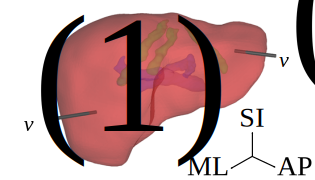
\includegraphics[width = 0.75\textwidth]{Images/Chapter3/Meshes3D/Meshes3D}%
\caption[Models of the liver anatomy]{Models of the liver boundary (capsule), large hepatic veins (green) and large portal veins (blue). The entry vectors are also indicated. The superior-inferior (SI), medial-lateral (ML), and anterior-posterior (AP) directions are shown.}
\label{fig:Meshes3D}
\end{figure*}

Two entry vectors $v^{(i)}$ were defined based on typical introducer placement for percutaneous RFA of liver tumors. Vector $v^{(1)}$ represents an intercostal approach into the right liver. Vector $v^{(2)}$ represents an anterior subcostal approach under the costal margin into the left liver. Both orientations reflect insertion under ultrasound guidance with the needle at 45 degrees to the transducer axis. 

For each $v^{(i)}$, the corresponding reachable workspace $R^{(i)}$ was measured by discretizing the liver volume $L$ (excluding the vasculature) into 4-mm voxels, and determining if each voxel could be reached by a permissible path. Paths that crossed the liver boundary (capsule) or vasculature were excluded to decrease risk of bleeding and other complications. Paths were also restricted to have one or two constant-curvature sections. Although insertion and rotation of a bent-tip steerable needle can theoretically generate more complex needle paths, in practice the mechanical properties of liver cause these complicated paths to relax into simpler paths. Two-section paths were excluded if the waypoint was already beyond the target (i.e., if the dot product of the vector from the waypoint to the target and the tangent vector at the waypoint was negative) to avoid impractical looping behavior. Finally, paths were excluded if they required radius of curvature below threshold $\rho$, which was varied as a parameter from 10-200~mm. Fig.~\ref{fig:Paths} shows examples of permissible and excluded paths. 

\subsection{Results}
\begin{figure*}[!t]
\centering
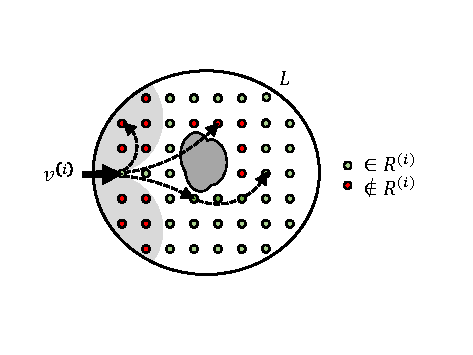
\includegraphics[width = 0.6\textwidth]{Images/Chapter3/Paths/Paths}%
\caption[Excluded and permissible paths]{Reachable and unreachable voxels within $L$, and lines showing, from left to right, an excluded path that violates $\rho$, an excluded path that passes through an obstacle, and a permissible two-part path.}
\label{fig:Paths}
\end{figure*}

Fig.~\ref{fig:ReachableSizeByRho} shows the size of the reachable set---specified by the ratio of the set sizes $\lvert R^{(i)} \rvert / \lvert L \rvert$---as a function of minimum radius of curvature $\rho$. With $\rho =$ 100~mm, paths starting at $v^{(1)}$ were able to reach approximately 8 percent of $L$, while paths starting at $v^{(2)}$ were able to reach approximately 41 percent of $L$. 

\begin{figure*}[!t]
\centering
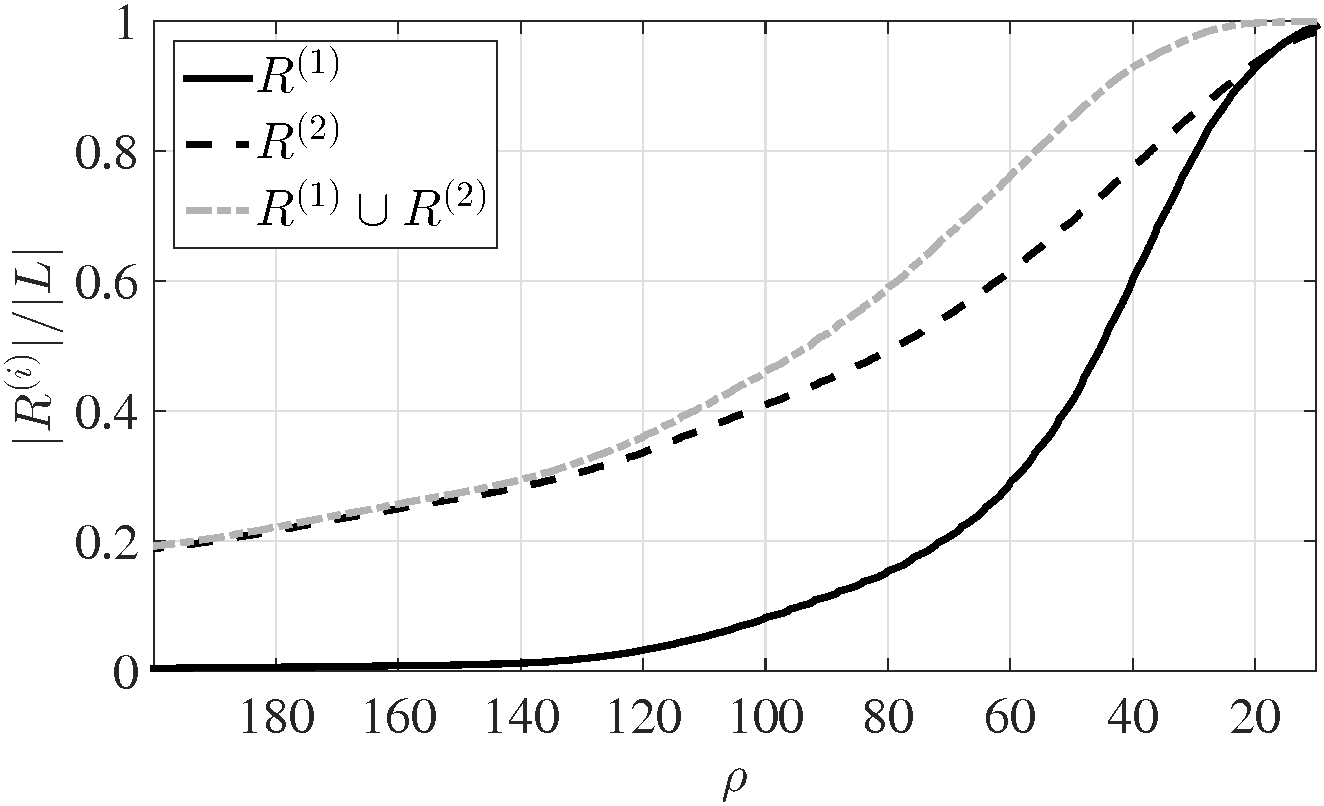
\includegraphics[width = 0.7\textwidth]{Images/Chapter3/ReachableSizeByRho/ReachableSizeByRho}%
\caption[Impact of radius of curvature on reachable set size]{Ratio of reachable set size to total liver size as a function of minimum radius of curvature $\rho$. Results for intercostal ($v^{(1)}$) and anterior approaches ($v^{(2)}$) are shown.}
\label{fig:ReachableSizeByRho}
\end{figure*}

Fig.~\ref{fig:FrontalSlice} shows a frontal slice near the center of the liver, with color indicating radius of curvature $\rho$ required to reach each voxel from $v^{(1)}$. The needle was not able to reach areas behind the hepatic veins and surrounding the insertion. Most of the slice was reachable using single-section paths, except for the area blocked by the vessels.

\subsection{Discussion}
Results shown in Fig.~\ref{fig:ReachableSizeByRho} reveal the gap between current needle steering methods and our clinical application. Most radius of curvatures values $\rho$ reported in biological tissue are between 100-200 mm [2]. Even combining the intercostal and anterior subcostal approaches, such needles would only permit access to 50 percent of the liver at best. Since the distribution of tumor sites is approximately uniform throughout the liver, current steerable needles would be unable to access many targets. Although angling the introducer could change the results shown in Fig. 4, interference from the ribs and potential for tissue injury limit this degree of freedom after initial insertion. 

An important potential advantage of needle steering in RFA of liver tumors is the ability to reach targets in the dome of the liver (on the right-lateral superior surface), which can be very difficult in some patients using traditional RFA probes due to interference from the ribs. As shown in Fig.~\ref{fig:FrontalSlice}, a radius of curvature of approximately 50~mm is necessary to reach the right-lateral aspect of the liver dome. We believe $\rho = 50$~mm is thus a reasonable curvature requirement for future development, since it allows the needle to access the liver dome, and reach approximately 85 percent of the liver volume from the entry points we have described.
  
\begin{figure*}[!t]
\centering
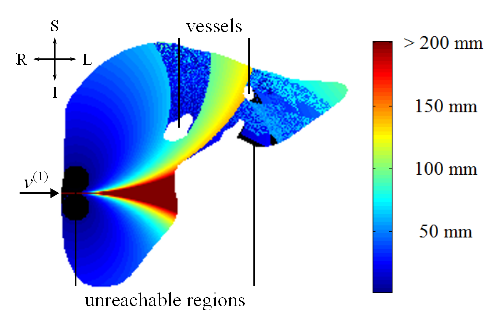
\includegraphics[width = 0.6\textwidth]{Images/Chapter3/FrontalSlice/FrontalSlice}%
\caption[Visualization of reachable set size]{Frontal slice of $L$. Colors indicate the radius of curvature $\rho$ required to reach each voxel. Black voxels were not reachable with any curvature in the examined range (10-200~mm). White voxels, including vessels inside the liver, were outside $L$.}
\label{fig:FrontalSlice}
\end{figure*}  


%-------------------------------------------------------------------------
\section{Analysis of Needle Tip Geometry }
%-------------------------------------------------------------------------
\label{sec:TipGeometryAnalysis}
\begin{figure}[!t]
\centering
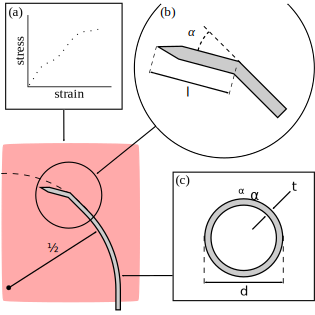
\includegraphics[width = 0.6\columnwidth]{Images/Chapter3/CurvatureFactors/CurvatureFactors}%
\caption[Factors impacting steerable needle curvature]{Factors impacting the radius of curvature $\rho$ of bent-tip steerable needles in liver tissue include (a) mechanical properties of the tissue (modeled as a hyperelastic solid), (b) tip geometry (defined by length $l$ and angle $\alpha$), and (c) needle material and cross section (defined by diameter $d$ and wall thickness $t$). In this chapter, we exclusively consider the impact of tip length $l$ and tip angle $\alpha$.}
\label{fig:NSFactors}
\end{figure}
As shown in Fig.~\ref{fig:NSFactors}, several factors affect the radius of curvature of steerable needles in tissue. In this dissertation we focus exclusively on the geometry of the bent tip. Bent-tip steerable needles described to date have generally had tip length $l \approx$~4~mm, and tip angle $\alpha \approx$~30~degrees~\cite{Patil2014,Swaney2013,Rucker2013,Majewicz2012}. Since bent-tip needles steer as a result of the asymmetric lateral force at the tip, it is reasonable to expect that a greater asymmetry---i.e., larger tip length $l$ or tip angle $\alpha$ as shown in Fig.~\ref{fig:NSFactors}---would result in improved curvature. However, because of the complex mechanics of needle-tissue interaction, it was unclear how altering tip parameters over a larger range of values than previously considered~\cite{Majewicz2010} would affect curvature performance. The work described in this section was meant to improve our understanding of the relationship between bent-tip geometry and radius of curvature. We proceeded in two ways. First, we used a simplified FE model of a bent tip moving in tissue to gain insight into the general relationship between tip length, tip angle, and steerable needle curvature. Second, we performed experimental testing to measure the actual needle radius of curvature $\rho$ achieved by bent-tip needles with different geometries in liver tissue.

Although some radius-of-curvature values in \textit{ex vivo} liver tissue have been reported close to or below our 50-mm requirement (our results in Chapter 3, and in~\cite{Majewicz2010}), the needles in these tests were solid Nitinol wires approximately 0.5~mm in diameter. These solid wires would be unable to deliver payloads such as contrast fluid, ethyl alcohol, or ablation leads. As we work towards early-stage clinical tests in the liver, steerable needle design requirements are increasingly driven by practical issues, such as the need to deliver a payload, or the need to pass through a rigid introducer sheath accessing the liver itself through layers of skin and fat.

\subsection{Finite-Element Model}
The physical interactions between a flexible steerable needle and soft tissue during insertion are extremely complex and difficult to approximate. In prior work, analytical methods~\cite{Misra2010} and FE models with cohesive elements~\cite{Misra2008} were used in an attempt to quantify tip forces and the resulting radius of curvature for bevel-tip steerable needles. Rather than create a more complicated model that encapsulates a bent-tip needle, in our current FE work, the goal was to use a simplified model to gain qualitative insight into the impact of the two specific parameters, bent-tip length and angle, on radius of curvature. As suggested in~\cite{Misra2010,Mahvash2001,Barbe2007}, continuous steerable needle insertion can be considered as a repeated discretized sequence of two steps. In the first step, the needle is inserted and deforms the tissue, resulting in forces at the needle tip and along the needle shaft. In the second step, the tissue ruptures. To make the FE modeling more tractable, we eliminated tissue rupture from the model, and only considered tissue loading. 

\begin{figure*}[!t]
\centering
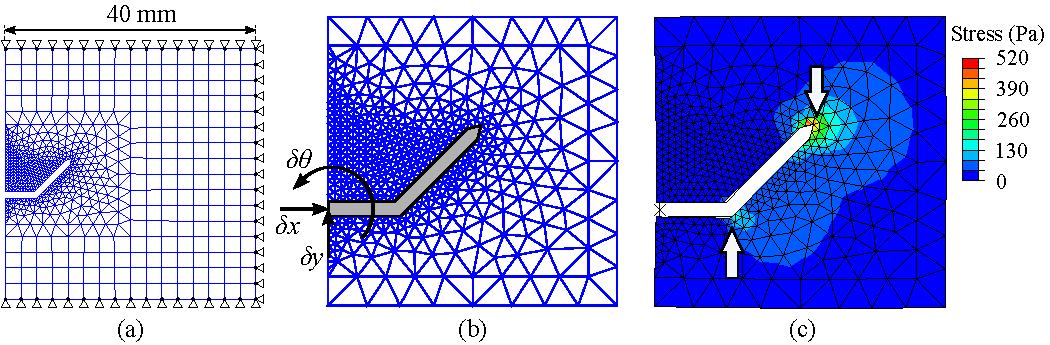
\includegraphics[width = \textwidth]{Images/Chapter3/Abaqus/Abaqus}%
\caption[Planar finite-element model of needle-tissue interaction]{Planar finite-element model of needle-tissue interaction: (a) The tissue was modeled as a square specimen with side length of 40~mm, with complete 3DOF constraints on three sides. A coarse quadrilateral mesh was used for most of the tissue, with a finer triangular mesh in the neighborhood of the needle tip. The needle tip was modeled as a rigid body, while the tissue was modeled as an incompressible hyperelastic solid. (b) The input to the model was horizontal displacement $\delta x$ of the needle. The output from the model was the rotation of the needle $\delta\theta$ and vertical displacement $\delta y$. These were used to calculate radius of curvature $\rho$. (c) After insertion, stress developed in the tissue, and was highest near the tip of the needle.}
\label{fig:Abaqus}
\end{figure*}

\begin{figure}[!t]
\centering
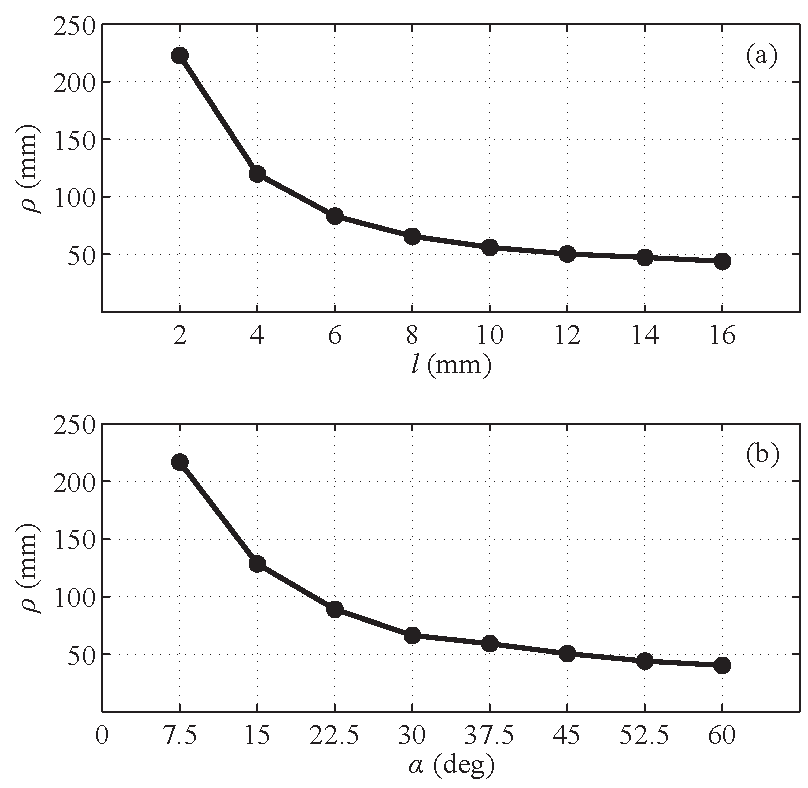
\includegraphics[width=0.6\columnwidth]{Images/Chapter3/AbaqusResults/AbaqusResults}%
\caption[Finite-element simulation results]{Finite-element simulation results: (a) Impact of bent-tip length $l$ on simulated radius of curvature $\rho$. (b) Impact of bent-tip angle $\alpha$ on simulated radius of curvature $\rho$.}
\label{fig:AbaqusResults}
\end{figure}

A 2D FE simulation was created using Abaqus Standard (Dassault Systemes; Velizy Villacoublay, France) with a static analysis step. The tissue was modeled as an incompressible hyperelastic solid, with Mooney-Rivlin coefficients as measured in~\cite{Kim2005}. A 40-mm square tissue specimen was modeled with its boundaries fully constrained on three sides, and free on the insertion face. The tissue was meshed with coarse quadrilateral elements (CPE4H), and finer triangular elements (CPE3H) in the contact region, as shown in Fig.~\ref{fig:Abaqus}. A mesh convergence test ensured the element size was sufficiently fine. Contact between the needle and tissue was modeled as frictionless as in~\cite{Misra2008}. Since bent-tip needles are generally created with inflexible steel or brass tips, the bent tip (including the distal 5~mm of the needle shaft) was modeled as a rigid body. The needle tip was free to translate in the $y$ direction and rotate. A linear torsional spring interaction was applied to the base of the rigid body, in order to model the needle shaft's resistance to bending. The spring constant was selected to yield $\rho = 120$~mm for a tip with $l = 4$~mm and $\alpha = 45$~degrees, since this radius of curvature is consistent with values described for similar steerable needle designs in the literature~\cite{Patil2014}, and with our experimental results as described below. The input to the simulation was the horizontal displacement of the needle tip $\delta x$, which was increased from 0.0~mm to 0.5~mm in a uniform ramp. The output of the simulation was the final vertical displacement $\delta y$ and rotation $\delta\theta$ of the bent tip after insertion. The radius of curvature $\rho$ was calculated by chaining together the $\delta x$, $\delta y$ and $\delta\theta$ displacement values obtained from the simulation, and fitting a circle to the resulting points.

\subsection{Finite-Element Results}
Fig.~\ref{fig:Abaqus}(c) shows an example of the FE model at the final simulation increment, with the resulting von Mises stresses in the simulated tissue overlaid on the deformed mesh. The largest stresses were seen around the tip of the needle, suggesting where tissue rupture might occur. Fig.~\ref{fig:AbaqusResults} summarizes FE results, with radius of curvature $\rho$ shown as a function of tip length $l$ and tip angle $\alpha$. Increases in both $l$ and $\alpha$ consistently resulted in reduced $\rho$, although only small reductions resulted beyond $l \approx 10$ mm and $\alpha \approx 45$~degrees.  

\begin{figure}[!t]
\centering
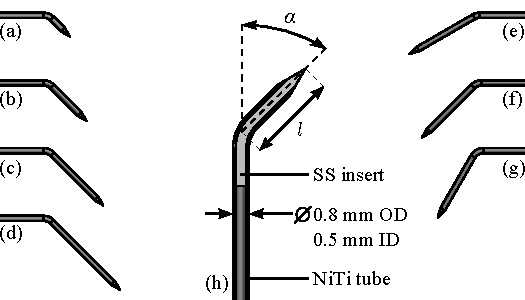
\includegraphics[width=0.65\columnwidth]{Images/Chapter3/Bent-TipGeometry/Bent-TipGeometry}%
\caption[Geometry of bent-tip steerable needles used for testing]{Geometry of bent-tip steerable needles used for testing in \textit{ex vivo} tissue. In the tip-length test, four needles with tip angle of 45 degrees and tip length of (a) 4~mm, (b) 8~mm, (c) 12~mm, and (d) 16~mm were tested. In the tip-angle test, three needles with tip length of 12~mm and tip angle of (e) 30~degrees, (f) 45~degrees, and (g) 60~degrees were tested. A schematic view (h) shows the construction of the bent-tip steerable needles. A Nitinol (NiTi) tube with outer diameter (OD) of 0.8~mm and inner diameter (ID) of 0.5~mm forms the shaft of each needle. A stainless-steel (SS) insert is bonded inside the tube with epoxy to form the tip. The tip is then ground into a cone using an abrasive wheel, and the tip is bent to the appropriate length and angle.}
\label{fig:Bent-TipGeometry}
\end{figure}

\subsection{Testing in \textit{Ex Vivo} Tissue}
In addition to FE simulations, we performed experimental tests in \textit{ex vivo} porcine liver tissue. We measured the impact of tip length $l$ and tip angle $\alpha$ by creating a number of steerable needles and separately varying those two parameters over a range of values. We inserted each needle into a tissue specimen, and measured the radius of curvature $\rho$ of the resulting needle path.

\subsubsection{Bent-Tip Needles}
Four steerable needles with tip angles $\alpha$ of 45~degrees and tip lengths $l$ of 4~mm, 8~mm, 12~mm, and 16~mm were created to test the impact of tip length. Three steerable needles with tip length $l$ of 12 mm and tip angle $\alpha$ of 30~degrees, 45~degrees, and 60~degrees were created to test the impact of tip angle. All the needles were created from Nitinol tubing with an outer diameter of 0.8~mm and an inner diameter of 0.5 mm, as shown in Fig.~\ref{fig:Bent-TipGeometry}.

\subsubsection{Insertion Protocol}
\textit{Ex vivo} porcine liver tissue obtained fresh from a local butcher was used to simulate human liver tissue. Each of the needles described above was inserted into a tissue specimen ten times, using the two-degree-of-freedom robot described in~\cite{Adebar2014}. The needles were inserted with constant velocity along minimum-radius-of-curvature paths; that is, they were inserted without any axial rotation so that the bent tip caused the needle to curve in a single direction. The insertion velocity was approximately 1.6 mm/s. A small incision in the capsule of the liver was used to introduce the needles, since the bent tips were too large for any available introducer sheath. The needles were inserted for a path length of approximately 100 mm, or until the tip of the needle exited the liver. 

\subsubsection{Ultrasound Imaging}
After insertion stopped, the needles were scanned using freehand 3D ultrasound imaging. A SonixMDP ultrasound system (Ultrasonix Research Corp.; Richmond, Canada) with a linear transducer was used to image the needle. This system includes a calibrated electromagnetic tracking system, which enables the collection of 3D ultrasound data. The imaging arrangement was exactly as described in~\cite{Greer2014}. To measure radius of curvature, the needle was segmented from the 3D ultrasound data by manually localizing the needle cross section in the 50 to 150 image frames captured from each insertion. In previous work~\cite{Adebar2014}, we found this manual segmentation to be repeatable to within approximately 0.5~mm. The radius of curvature of the needle was measured by reducing the segmentation points to two dimensions using singular value decomposition, identifying the circular arc that best fit the 2D segmentation points in the least-squares sense, and determining the radius of the arc. The steerable needle's path was generally very close to lying in a plane; across all tests the average distance of the 3D segmentation points from the reduced 2D points was approximately 0.3 mm.

\begin{figure}[!t]
\centering
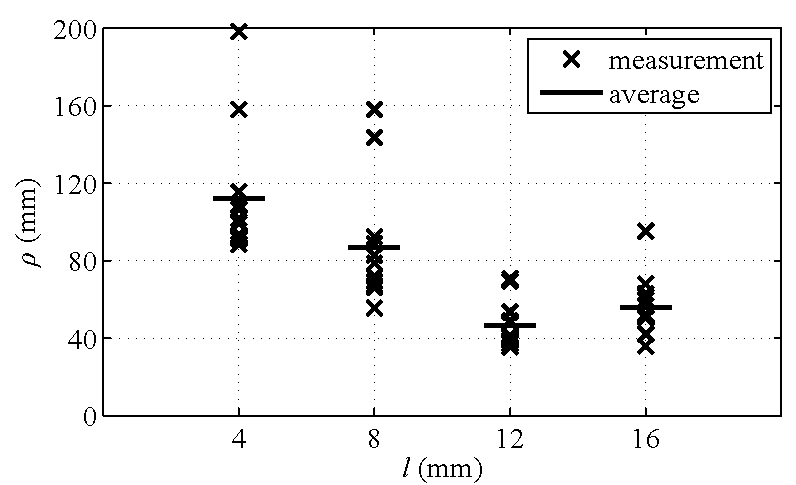
\includegraphics[width=0.6\columnwidth]{Images/Chapter3/CurvatureVsLength/CurvatureVsLength}%
\caption[Impact of bent-tip length on needle radius of curvature]{Summary of experimental results showing impact of bent-tip length $l$ on needle radius of curvature $\rho$ in \textit{ex vivo} tissue. Four tip lengths (4 mm, 8 mm, 12 mm, and 16 mm) were tested. All measured values of $\rho$ are shown, along with average values $\rho_{\text{avg}}$ for each value of $l$.}
\label{fig:CurvatureVsLength}
\end{figure}

\begin{figure}[!t]
\centering
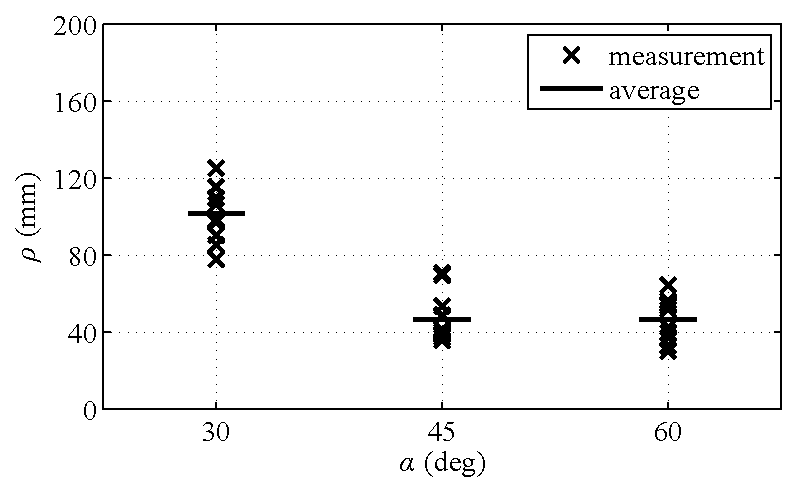
\includegraphics[width=0.6\columnwidth]{Images/Chapter3/CurvatureVsAngle/CurvatureVsAngle}%
\caption[Impact of bent-tip angle on needle radius of curvature]{Summary of experimental results showing impact of bent-tip angle $\alpha$ on needle radius of curvature $\rho$ in \textit{ex vivo} liver tissue. Three tip angles (30 degrees, 45 degrees, and 60 degrees) were tested. All measured values of $\rho$ are shown, along with average values $\rho_{\text{avg}}$ for each value of $\alpha$.}
\label{fig:CurvatureVsAngle}
\end{figure} 

\subsection{Results in \textit{Ex Vivo} Tissue}
Fig.~\ref{fig:CurvatureVsLength} summarizes the measured radius-of-curvature values as a function of the tip length. Average radius of curvature $\rho_{\text{avg}}$ (mean~$\pm$~standard deviation) for $l =$~4~mm, 8~mm, 12~mm and 16~mm was 112.1~$\pm$~33.0~mm, 86.8~$\pm$~31.8~mm, 46.8~$\pm$~12.2~mm and 55.8~$\pm$~15.4~mm respectively. Tip length $l$ of 12 mm resulted in the smallest average radius of curvature, as well as the least variability in curvature. 

Fig.~\ref{fig:CurvatureVsAngle} summarizes the measured radius-of-curvature values as a function of the tip angle. Average radius of curvature $\rho_{\text{avg}}$ (mean~$\pm$~standard deviation) for $\alpha =$~30~degrees, 45~degrees and 60~degrees was 101.4~$\pm$~13.6~mm, 46.8~$\pm$~12.2~mm, and 46.7~mm~$\pm$~10.7~mm respectively. Tip angle $\alpha$ of 60 degrees resulted in the smallest average radius of curvature, although there was substantial variability. Tip angle $\alpha$ of 45 degrees resulted in slightly higher average radius of curvature, but with much less variability.

Fig.~\ref{fig:CurvatureVsLengthData} shows the segmentation results and best-fit circular arcs from the tip-length test. Fig.~\ref{fig:CurvatureVsAngleData} shows the segmentation results and best-fit circular arcs from the tip-angle test.  

\begin{figure*}[!t]
\centering
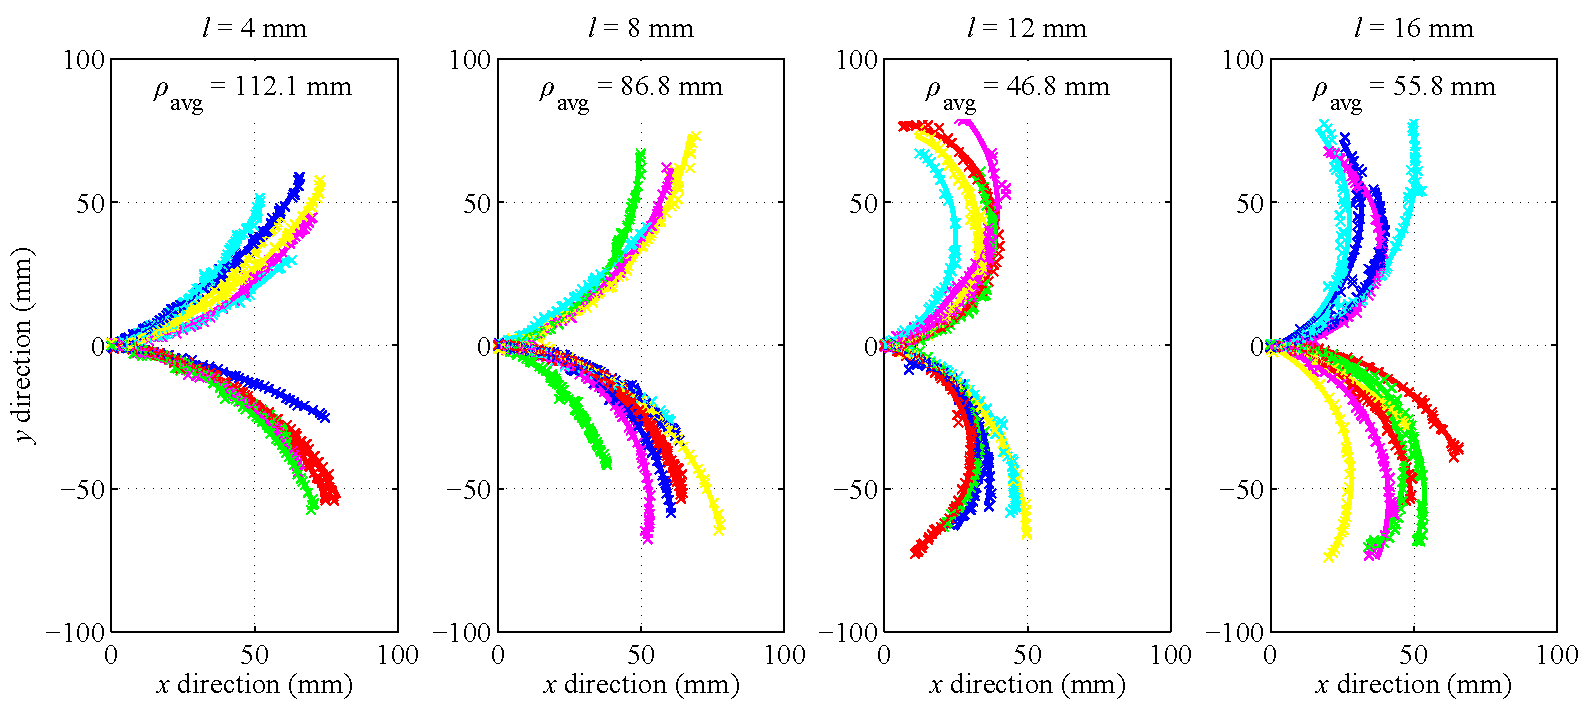
\includegraphics[width=\textwidth]{Images/Chapter3/CurvatureVsLength/CurvatureVsLengthData}%
\caption[Experimental results showing impact of bent-tip length]{Experimental results showing impact of bent-tip length $l$ on needle radius of curvature $\rho$ in \textit{ex vivo} tissue. Four tip lengths (4 mm, 8 mm, 12 mm, and 16 mm) were tested. All segmentation results and average values $\rho_{\text{avg}}$ for each value of $l$ are shown. The needle paths have been moved to a common origin for comparison.}
\label{fig:CurvatureVsLengthData}
\end{figure*}

\begin{figure*}[!ht]
\centering
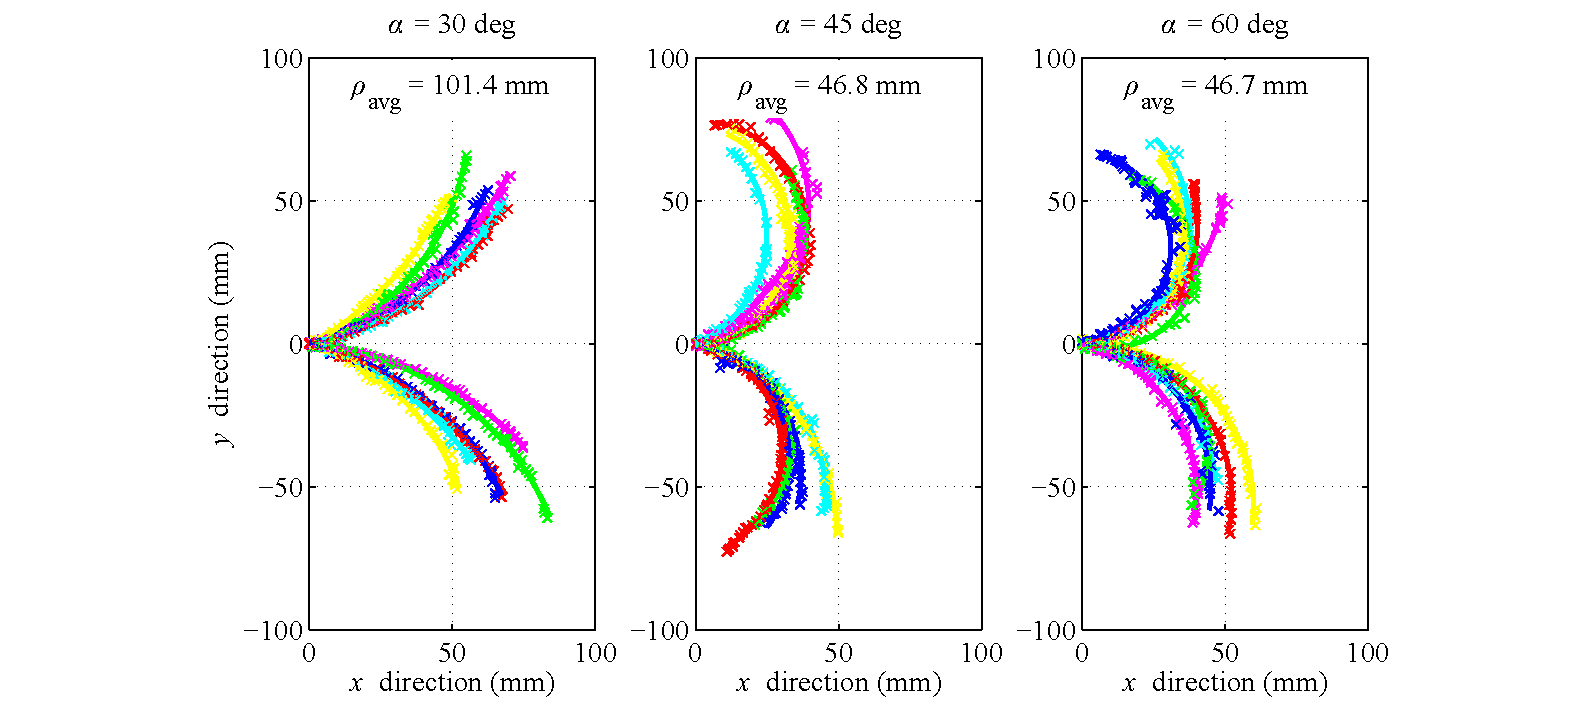
\includegraphics[width=\textwidth]{Images/Chapter3/CurvatureVsAngle/CurvatureVsAngleData}%
\caption[Experimental results showing impact of bent-tip angle]{Experimental results showing impact of bent-tip angle $\alpha$ on needle radius of curvature $\rho$ in \textit{ex vivo} liver tissue. Three tip angles (30 degrees, 45 degrees, and 60 degrees) were tested. All segmentation results and average values $\rho_{\text{avg}}$ for each value of $\alpha$ are shown. The needle paths have been moved to a common origin for comparison.}
\label{fig:CurvatureVsAngleData}
\end{figure*}

\subsection{Discussion}
In the \textit{ex vivo} tip-length test, the needle with $l =$~4~mm and $\alpha =$~45~degrees showed similar radius-of-curvature values to those previously reported using equivalent bent-tip steerable needles in liver tissue~\cite{Patil2014,Swaney2013}. This is expected, since the needles used in those tests had similar tip and shaft geometries to our needles. The needles with $l =$~4~mm and $l =$~8~mm showed more variability in curvature (the needle would occasionally follow a much less tightly curved path) than the needles with $l =$~12~mm and $l =$~16~mm. It may be that the heterogeneous liver tissue affects needles with smaller tip lengths more strongly, as they generate less lateral force to compensate for small vessels, fascia, etc.\ in the liver tissue. A previous study also showed a large amount of variability in radius of curvature using steerable needles with 4-mm tips~\cite{Majewicz2010}.

During insertion, the needle with $\alpha =$~60~degrees showed some undesirable behavior, as the needle tip tended to catch on membranes or small vessels. The jerky motion of the needle tip as it hung on obstacles before piercing through was not seen frequently with other tip geometries, and would be undesirable in a clinical setting.

The \textit{ex vivo} test results and the FE simulation results generally agreed well. For tip length, the \textit{ex vivo} radius-of-curvature results were within approximately 10~mm of the FE results, except for $l = 8$~mm, where the FE simulation predicted $\rho$ approximately 20~mm smaller than the \textit{ex vivo} result. Unlike the FE simulation results---where $\rho$ was approximately equal for $l = 12$~mm and $l = 16$~mm---in the \textit{ex vivo} test results, $\rho$ increased by approximately 9.0~mm on average going from $l = 12$~mm to $l = 16$~mm. This may be the impact of factors that were not considered in our FE simulation, such as tissue rupture mechanics or needle-tissue friction. For tip angle, the \textit{ex vivo} radius-of-curvature results were within approximately 5~mm of the FE results, except for $\alpha = 30$~degrees, where the FE simulation predicted $\rho$ approximately 35~mm smaller than the \textit{ex vivo} result. Overall both the \textit{ex vivo} test results and the FE simulation results showed that bent-tip steerable needles with $l >$~4~mm and $\alpha >$~30~degrees can achieve substantially smaller radius of curvature. The \textit{ex vivo} test results in particular showed that with $l =$~12~mm and $\alpha =$~45~degrees, a 0.8-mm tubular Nitinol needle can achieve $\rho$ as small as 50~mm in liver tissue.

\section{Articulated-Tip Needle}
\label{sec:Articulated-TipNeedle}
Two important practical issues preclude the clinical application of steerable needles having rigid bent tips with $l =$~12~mm and $\alpha =$~45~degrees in percutaneous RFA of liver tumors. The first issue relates to the introducer sheath, which is a separate rigid needle required to puncture layers of skin and fat to access the liver itself. A bent-tip needle with $l >$~4~mm and $\alpha >$~30~degrees cannot fit through a realistic introducer sheath, since a typical 15-gauge introducer has an inner diameter of approximately 1.5~mm. The second issue relates to rotation of the needle during insertion, which is necessary for control of the steerable needle. Rotation of a bent-tip needle results in deformation of the tissue immediately surrounding the tip. As $l$ and $\alpha$ increase, there is more tissue deformation, resulting in decreased targeting accuracy and potentially greater tissue damage. There is also more resistance to rotation with longer tips, potentially increasing torsional deflection, which has previously been shown to be problematic for needle control~\cite{Reed2009}.

Motivated by these issues, we created a new articulated-tip steerable needle. Our implementation is essentially a bent-tip steerable needle with an actuated one-degree-of-freedom rotary joint. The articulated-tip steerable needle switches between a straight needle, which can pass through an introducer and rotate, and a bent-tip needle, which can achieve clinically relevant radius of curvature in liver tissue.

As mentioned in Chapter 1, multiple designs for steerable needles with articulating sections have been proposed. Several groups have described using SMA actuators to articulate steerable needle sections~\cite{Ayvali2012,Datla2014,Ryu2014}. While these designs are promising, further refinement is still needed to improve miniaturization, actuation force, and response time. Our design is more similar to the needles described by Swaney et al.~\cite{Swaney2013}, who use a passive one-degree-of-freedom flexure tip, and van de Berg et al.~\cite{vandeBerg2015}, who use a short conical tip with an active two-degree-of-freedom ball-and-socket joint. Our needle design is unique in its use of exaggerated tip geometry to achieve tightly curved paths in biological tissue.

The mechanical design and experimental validation of our articulated-tip needle are described in the remainder of this section.

\subsection{Design}
\subsubsection{Articulated Tip}
The articulated-tip mechanism is shown in Fig.~\ref{fig:ArticulatedTipDetail}. The mechanism consists of a two-piece 3D-printed hinge, secured by a 0.25-mm stainless-steel pin. The hinge material is MicroFine Green, a proprietary ABS-like material that allows a stereolithography process with a feature resolution of 0.05 mm (Protolabs Inc; Maple Plain, MN). The proximal hinge section mates to a 0.8-mm tubular Nitinol shaft, and is secured with epoxy adhesive. Similarly, the distal hinge section mates to a ground conical stainless-steel tip, and is again secured with epoxy adhesive. Conical tips were selected, rather than the bevel tips commonly seen in prior bent-tip needle steering work~\cite{Majewicz2012,Majewicz2010}, because it was easier to make them extremely sharp using our grinding wheel setup. 

\begin{figure*}[!ht]
\centering
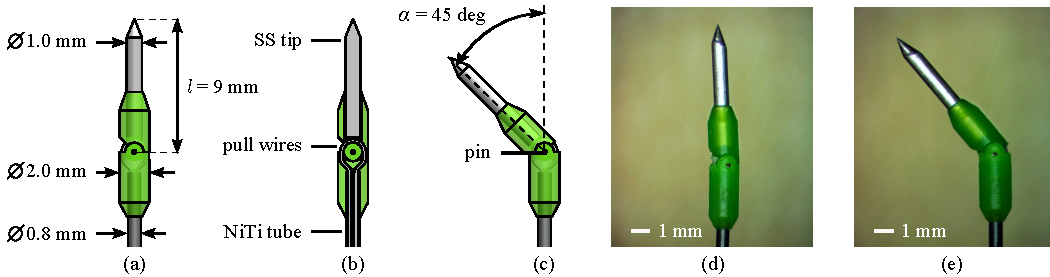
\includegraphics[width=\textwidth]{Images/Chapter3/ArticulatedTipDetail/ArticulatedTipDetail}
\caption[Articulated-tip needle mechanism]{The articulated-tip needle mechanism: (a) Schematic of the articulated tip in the straight configuration. The tip consists of a two-part 3D-printed hinge mechanism approximately 2.0 mm in diameter, secured to a 0.8-mm Nitinol tube, and a 1.0-mm ground stainless-steel tip. (b) Section view of the articulated tip in the straight configuration. A single continuous, pretensioned Nitinol pull wire is used to articulate the needle tip. The pull wire runs through the tubular Nitinol (NiTi) needle shaft, through channels in the proximal hinge section, and is secured to the distal hinge section with adhesive. A ground conical stainless-steel (SS) tip is secured to the distal hinge section with adhesive. (c) Schematic of the articulated-tip in the bent configuration. Nominal tip parameters of $l =$ 9~mm and $\alpha =$ 45~degrees were selected. (d) Micrograph of the assembled tip in the straight configuration. (e) Micrograph of the assembled tip in the bent configuration.}
\label{fig:ArticulatedTipDetail}
\end{figure*} 

A 0.13-mm Nitinol pull wire runs through the length of the needle shaft, through channels in the proximal hinge section, and is secured to the distal hinge section using epoxy adhesive. This pull wire is wound around a cable pulley in the needle hub, as described below, and allows actuation of the articulated tip. For reasons we describe in Section~\ref{sec:ArticDiscussion}, the articulated-tip needle is switched between fully straight and fully bent. Contact between the mating hinge components limits the range of motion in both directions. In the current design, tip length $l$ is 9~mm, while tip angle $\alpha$ is approximately 45 degrees. (Because of the manufacturing tolerances of the hinge components the actual maximum value of $\alpha$ was about 3 degrees less than the nominal value.) This tip geometry was selected based on the results of Section~\ref{sec:TipGeometryAnalysis}, and the strength limits of the plastic hinges. Although bent-tip needles with $l = 12$~mm had the smallest average radius of curvature in Section~\ref{sec:TipGeometryAnalysis}, the plastic hinge material was not able to support such long tips without occasionally failing.

\begin{figure*}[!h]
\centering
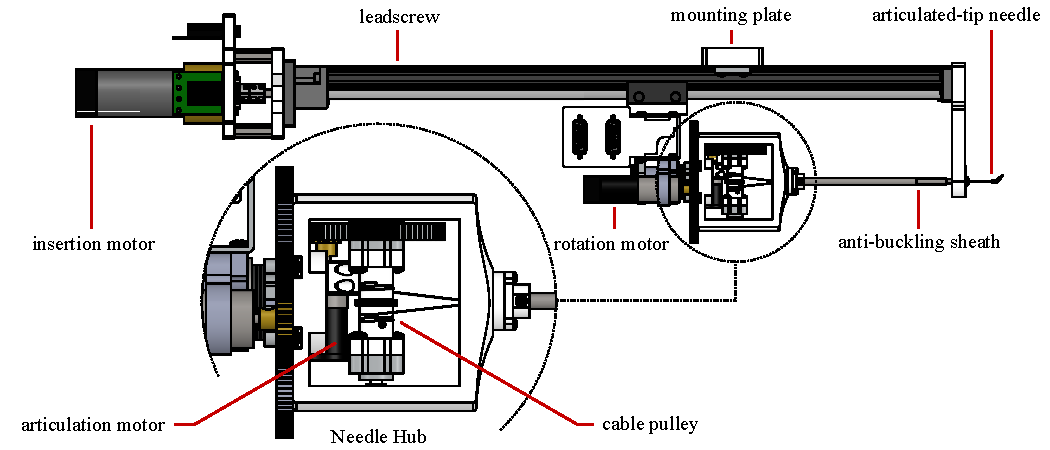
\includegraphics[width=0.6\textwidth]{Images/Chapter3/NS2Robot/NS2Robot}
\caption[Top view of the articulated-tip robot]{Schematic top view of the articulated-tip needle steering robot. DC motors drive a leadscrew for insertion of the needle, a rotary stage for rotation of the needle, and a cable pulley for articulation of the tip. A telescoping sheath prevents the flexible steerable needle from buckling outside of tissue. A detail view shows the removable needle hub attached to the rotatory stage. The needle steering robot is attached to a passive positioning arm using a mounting plate. A standard introducer sheath and connecting luer-lock fixture are omitted.}
\label{fig:NS2Robot}
\end{figure*}

\subsubsection{Needle Hub}
Fig.~\ref{fig:NS2Robot} includes a detail view of the articulated-tip steerable needle hub. The needle hub is a 3D-printed shell that mates to the rotary platform of the needle steering robot. Within the hub is a bearing-mounted cable pulley attached to a spur gear. The spur gear meshes with a pinion gear driven by a DC motor mounted on the rotary platform. The steerable needle shaft and anti-buckling sheath are also both affixed to the needle hub, and the entire needle/sheath assembly is removable from the needle steering robot.

\subsubsection{Needle Steering Robot}
Fig.~\ref{fig:NS2Robot} shows a schematic overview of the new robot designed to drive articulated-tip steerable needles. The robot is similar to the one described in~\cite{Majewicz2012}, but with an additional degree of freedom for the active articulation of the needle tip. The robot incorporates three DC motors: one drives a leadscrew for insertion of the needle, one drives a rotary platform that allows rotation of the needle hub, and one drives the cable pulley that allows articulation of the needle tip. A clamping plate allows the entire needle steering robot to be mounted on a passive positioning arm, which is attached to the standard rails on an operating room table. 

\subsection{Experimental Validation}

\subsubsection{Method}
\textit{Ex vivo} porcine liver tissue obtained fresh from a local butcher was used to simulate human liver tissue in all testing of the articulated-tip needle. Fig.~\ref{fig:ExperimentalSetupArticulatedTip} shows the experimental setup used in validation testing. We evaluated our articulated-tip steerable needle design in three ways. 

\begin{figure}[!t]
\centering
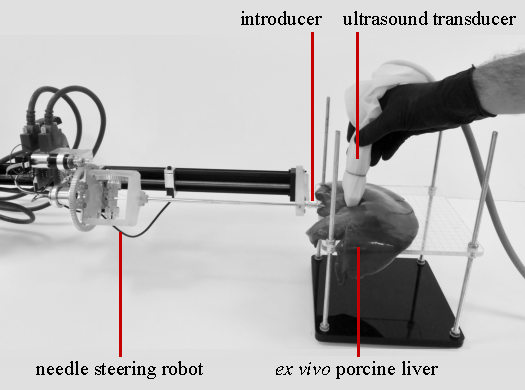
\includegraphics[width=0.6\columnwidth]{Images/Chapter3/ExperimentalSetup/ExperimentalSetup}
\caption[Setup for validation testing of the articulated-tip needle]{Experimental setup for validation testing of the articulated-tip steerable needle. The needle steering robot is mounted on a passive positioning arm. \textit{Ex vivo} porcine liver was used to simulate human liver tissue. The articulated-tip needle entered the liver tissue through a 13-gauge introducer sheath. A tracked 2D ultrasound transducer was used to image the needle for validation. }
\label{fig:ExperimentalSetupArticulatedTip}
\end{figure} 

First, to evaluate the articulation mechanism, the tip angle in the bent configuration was compared in free space and in liver tissue. To evaluate the tip angle in free space, the tip was imaged using a microscope with a digital camera attachment. The distal tip section and needle shaft were manually segmented from the micrograph, and the tip angle was measured. To evaluate the angle in tissue, the tip was articulated under 2D ultrasound imaging. The distal tip section and needle shaft were manually segmented from the ultrasound images, and the tip angle was measured.

Second, to evaluate the radius of curvature achieved by the articulated-tip needle, we performed a number of minimum-radius-of-curvature insertions (i.e., insertions with the tip kept in the bent configuration) in liver tissue. Each insertion was performed in a new section of liver to keep the needle from following an established track. After insertion stopped, the needles were scanned and segmented using the same method described in Section~\ref{sec:TipGeometryAnalysis} for the bent-tip needles.

Finally, we compared the articulated-tip needle design with bent-tip needles in a practical task, by performing a direction change maneuver with both needles. In this maneuver, the needle was inserted along a straight path for approximately 40~mm, before being steered with minimum radius of curvature in one direction for an additional 40~mm. The bent-tip needle was steered along the straight path using open-loop duty-cycle control, while the articulated-tip needle was inserted in the straight configuration. The needle was scanned and segmented after both the initial and final insertion steps, and the maximum deviation $\delta$ from the initial vector was measured. The bent-tip needle was the largest needle from Section~\ref{sec:TipGeometryAnalysis} that would fit through a 13-gauge introducer, with dimensions $l =$~4~mm and $\alpha =$~45~degrees (needle (a) in Fig.~\ref{fig:Bent-TipGeometry}).  

\begin{figure}[!t]
\centering
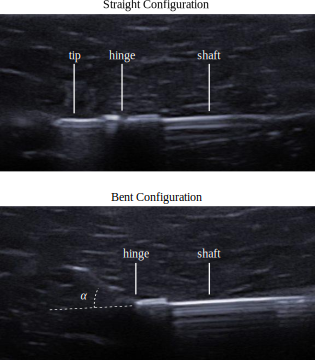
\includegraphics[width = 0.65\columnwidth]{Images/Chapter3/ArticulatedTipUS/ArticulatedTipUS}%
\caption[Ultrasound images of the articulated tip]{Ultrasound images of the articulated tip demonstrate the ability of the needle to achieve the straight (top) and bent (bottom) configurations in \textit{ex vivo} liver tissue. In the bent configuration, tip angle $\alpha$ was found to be 41.5 degrees using manual segmentation.}
\label{fig:ArticulatedTipUS}
\end{figure}

\begin{figure}[!t]
\centering
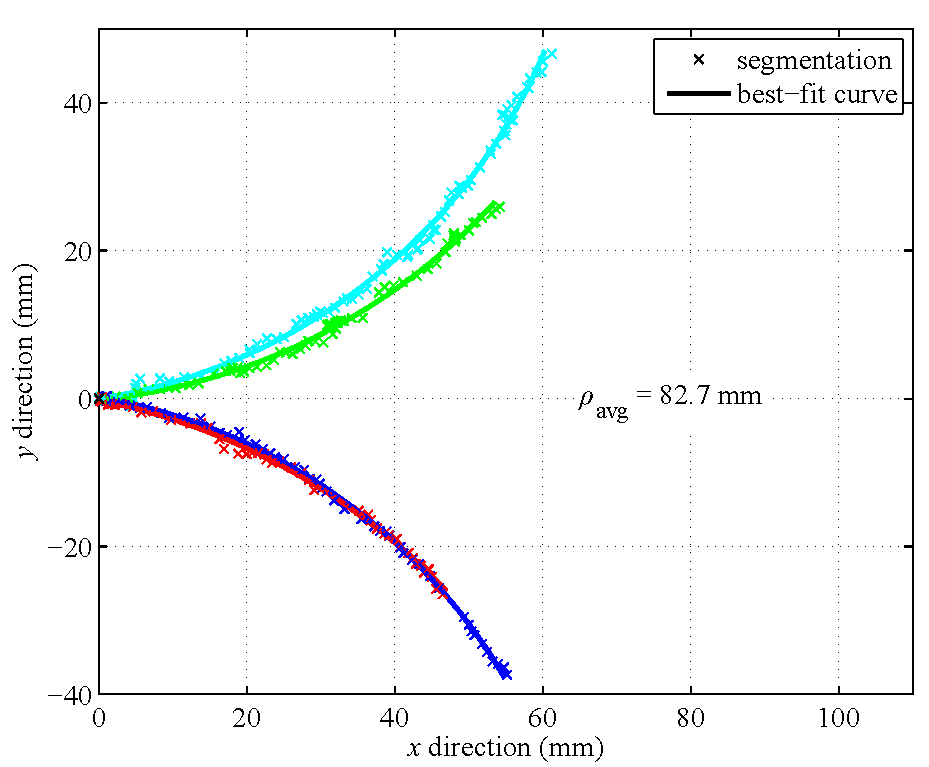
\includegraphics[width=0.75\columnwidth]{Images/Chapter3/ArticulatedTipMaxCurvature/ArticulatedTipMaxCurvature}
\caption[Minimum-$\rho$ results with the articulated-tip needle]{Minimum-radius-of-curvature results with the articulated-tip steerable needle. The needle was inserted with the articulated-tip in the bent configuration. Across four trials in fresh sections of \textit{ex vivo} liver tissue, the average radius of curvature $\rho_{\text{avg}}$ was 82.7~mm. The needle paths have been moved to a common origin for comparison.}
\label{fig:ArticulatedMaxCurvature}
\end{figure}  

\begin{figure*}[!ht]
\centering
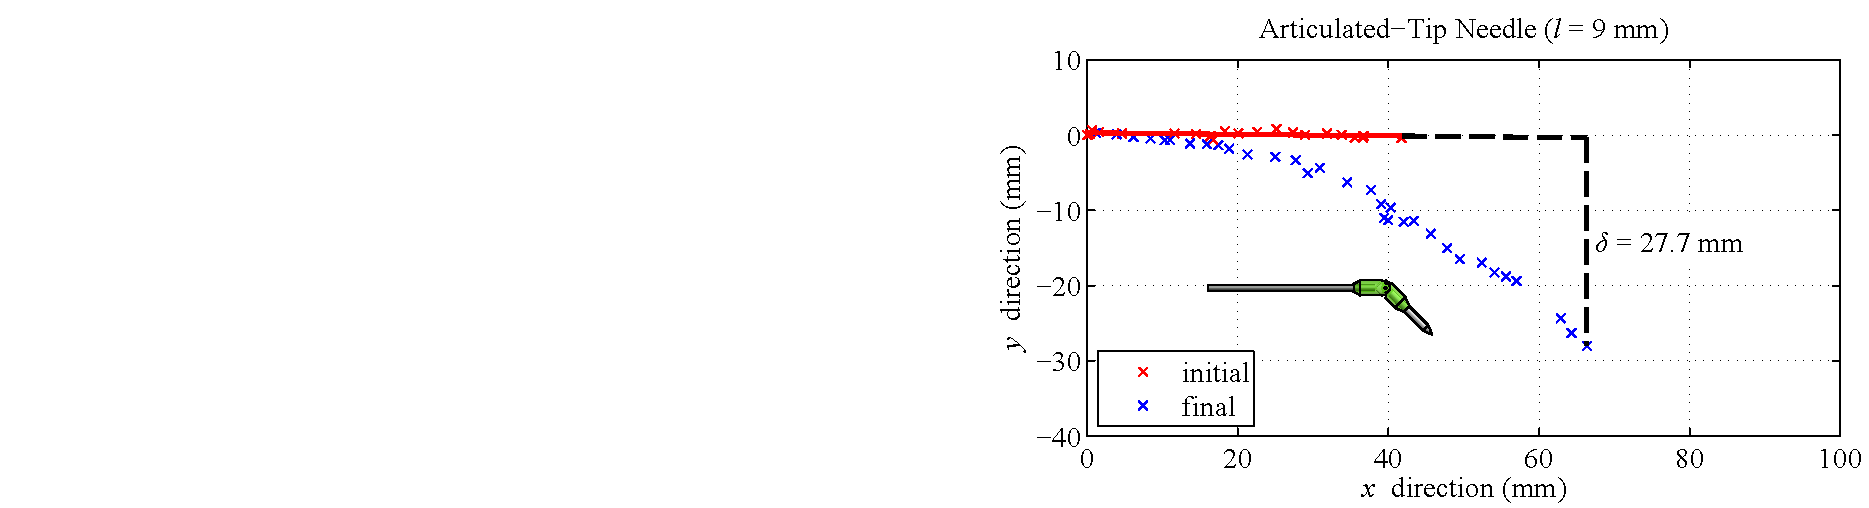
\includegraphics[width=0.75\textwidth]{Images/Chapter3/InsertAndTurn/InsertAndTurn1}
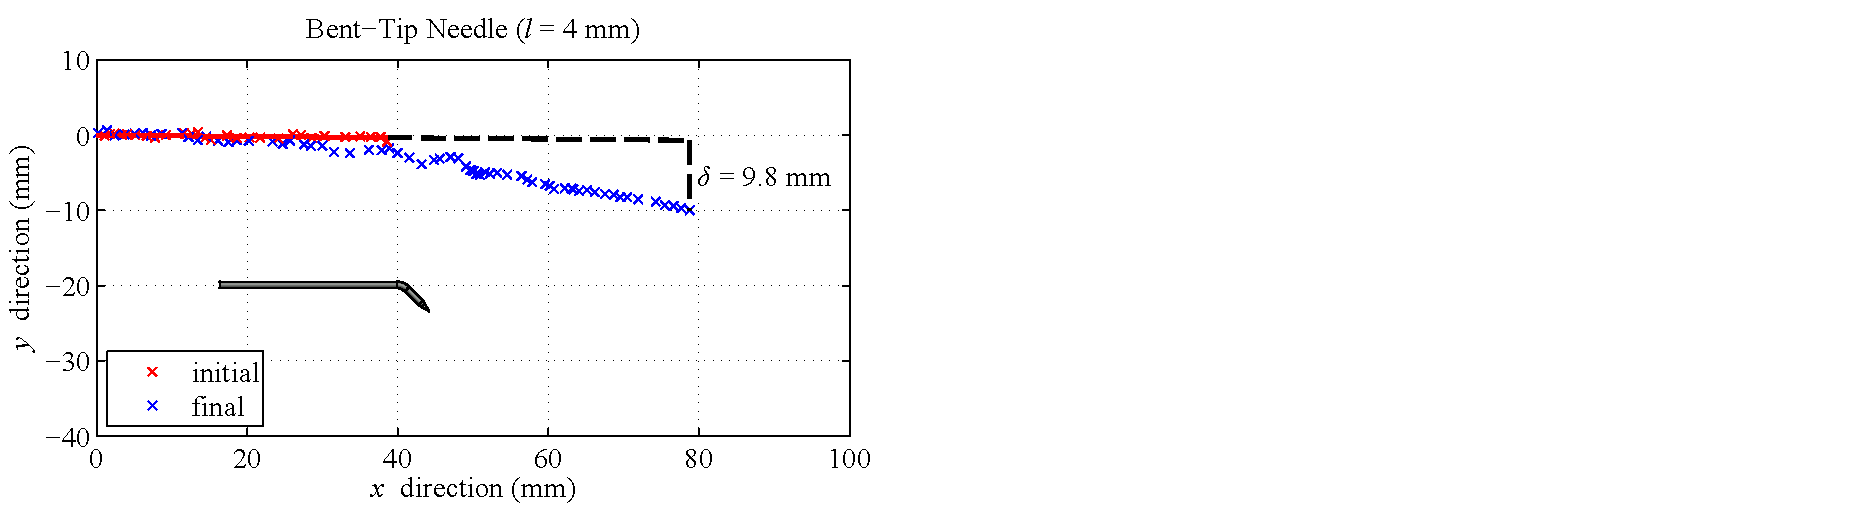
\includegraphics[width=0.75\textwidth]{Images/Chapter3/InsertAndTurn/InsertAndTurn2}
\caption[Maneuvers using bent-tip and articulated-tip needles]{Representative examples of direction change maneuver using a bent-tip needle with $l =$~4~mm and $\alpha =$~45~degrees, and an articulated-tip needle with $l =$~9~mm and $\alpha \approx$~45~degrees. Each needle was inserted along a straight path for approximately 40~mm, then was steered along the minimum-radius-of-curvature path for an additional 40~mm. In the maneuvers shown in the figure, deviation $\delta$ was 9.8~mm using the bent-tip needle, and 27.7~mm using the articulated-tip needle.}
\label{fig:InsertAndTurn}
\end{figure*}

\subsubsection{Results}
Fig.~\ref{fig:ArticulatedTipUS} shows ultrasound images of the articulated-tip needle in the straight and bent configurations. The needle steering robot was able to consistently articulate the needle tip to the same extent in tissue as in free space. In the micrographs shown in Fig.~\ref{fig:ArticulatedTipDetail}, the measured tip angle $\alpha$ was 41.1~degrees, while in the ultrasound images shown in Fig.~\ref{fig:ArticulatedTipUS}, the measured tip angle $\alpha$ was 41.5~degrees.

Fig.~\ref{fig:ArticulatedMaxCurvature} shows maximum curvature results for an articulated-tip needle with tip length $l =$~9~mm and tip angle $\alpha =$~45~degrees. Over the four tests shown in Fig.~\ref{fig:ArticulatedMaxCurvature}, the mean curvature was 82.7~mm with a standard deviation of 4.9~mm.       

Fig.~\ref{fig:InsertAndTurn} shows segmentation results from representative examples of the direction change maneuver. Using a bent-tip steerable needle, the maximum deviation $\delta$ from the initial vector was 9.8~mm for the test shown. Using the articulated-tip steerable needle, the maximum deviation $\delta$ was 27.7~mm for the test shown. It can be seen in Fig.~\ref{fig:InsertAndTurn} that the proximal 40~mm of each steerable needle shaft was displaced after the direction change maneuver. The Nitinol needle shafts, which were stiffer than the surrounding liver tissue, relaxed into single smooth circular curves rather than forming segmented straight-to-curved paths. The relaxation of the needle shaft was especially visible for the articulated-tip needle, which exhibited greater displacement $\delta$ from the initial vector.

\subsection{Discussion}
\label{sec:ArticDiscussion}
Overall, the validation results described above demonstrate that an articulated-tip needle is able to achieve better curvature in liver tissue than the largest practical bent-tip needle ($l \approx$~4~mm). However, there are several issues with the current design, mostly related to construction of the miniature hinges, which we plan to address before applying the design in an animal model. In the current design, the hinge elements are an ABS-like plastic. We are currently exploring machining methods that will allow us to create stainless-steel hinge elements, in order to improve performance, robustness and biocompatibility. Because of their plastic construction, the current hinges occasionally fail if tip lengths longer than about 9~mm are used. Based on the results of Section~\ref{sec:TipGeometryAnalysis}, increasing the tip length to approximately 12~mm should reduce radius of curvature to meet the 50-mm design requirement for our procedure. The current design is also sized to pass through a 13-gauge introducer sheath. The overall diameter will need to be slightly reduced to pass through a 15-gauge introducer sheath, which is the largest size that is clinically acceptable for percutaneous RFA of liver tumors.

Unlike in the design of van de Berg et al.~\cite{vandeBerg2015}, in our current design we elected to actuate the tip in a binary sense at the limits of the range of travel (i.e., the needle tip is either fully straight or fully bent). This simplifies the control of actuation, since we no longer need to compensate for the compliance of the pull wires. 

Based on observing the needle under ultrasound imaging during articulation, the moving tip easily displaces the liver tissue, making it unlikely that tissue damage is occurring due to tissue stress in the lateral direction. Confirming this would require a detailed histological analysis, which is beyond the scope of this dissertation. During closed-loop image-guided needle steering, the articulated-tip needle is only rotated in the straight configuration. When the needle is curving in one direction and the steering control software (not described in this dissertation) determines the needle should curve in a different direction, insertion stops, the needle is switched to the straight configuration, the needle is rotated to the new desired orientation, the needle is switched to the bent configuration, and insertion continues. A more detailed analysis of schemes for closed-loop image-guided control of the articulated-tip needle will be the subject of future work.

Both the flexure-tip design described by Swaney et al.~\cite{Swaney2013} and the ball-and-socket design described by van de Berg et al.~\cite{vandeBerg2015} could potentially be used with the exaggerated tip geometries we have described. It is unclear how well the passive flexure-tip needle, which relies on an asymmetric bevel to achieve articulation, would work for larger tip lengths and tip angles. The passive flexure also requires duty-cycle control to achieve straight paths, which introduces practical issues such as sensor windup and torsional needle deflection. Active articulated tips can also be used to introduce recognizable motion signatures into medical image data, as in~\cite{Adebar2014}, in order to reduce the complexity of image segmentation.

